\documentclass[12pt]{article}
\usepackage[utf8]{inputenc}
\usepackage[russian]{babel}
\usepackage{graphicx}
\usepackage{subcaption}
\graphicspath{ {./images/} }


\begin{document}

Дубровских Никита 221-361

\textit{\textbf{Вариант 7}}

\textit{\textbf{Задание 20.}}

\textit{Орграф задан матрицей смежности. Необходимо:}\\
\textit{a) нарисовать граф;}\\
\textit{б) заменить все дуги ребрами и в полученном неориентированном графе найти
эйлерову цепь (или цикл);}\\
\textit{в) провести раскраску графа и найти его хроматическое число}\\

\begin{center}
	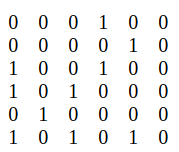
\includegraphics[scale=.8]{20.png}
\end{center}

\underline{Решение:}

а) Нарисуем граф:

\begin{center}
	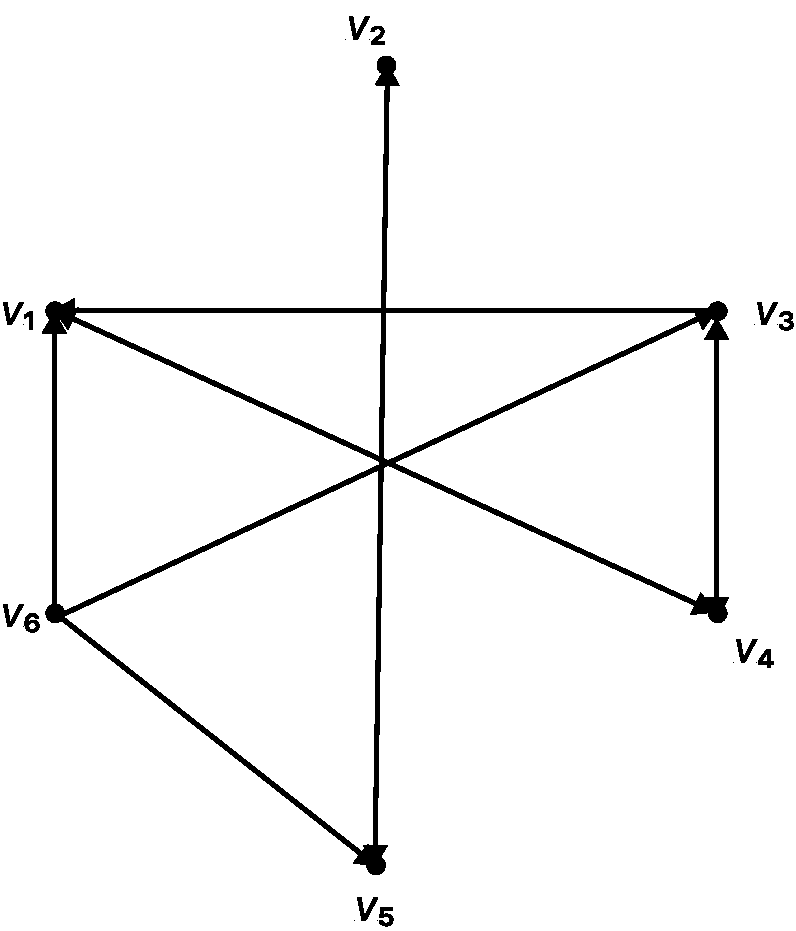
\includegraphics[scale=.8]{20_1.pdf}
\end{center}

б) Заменим все дуги ребрами. Получим:

\begin{center}
	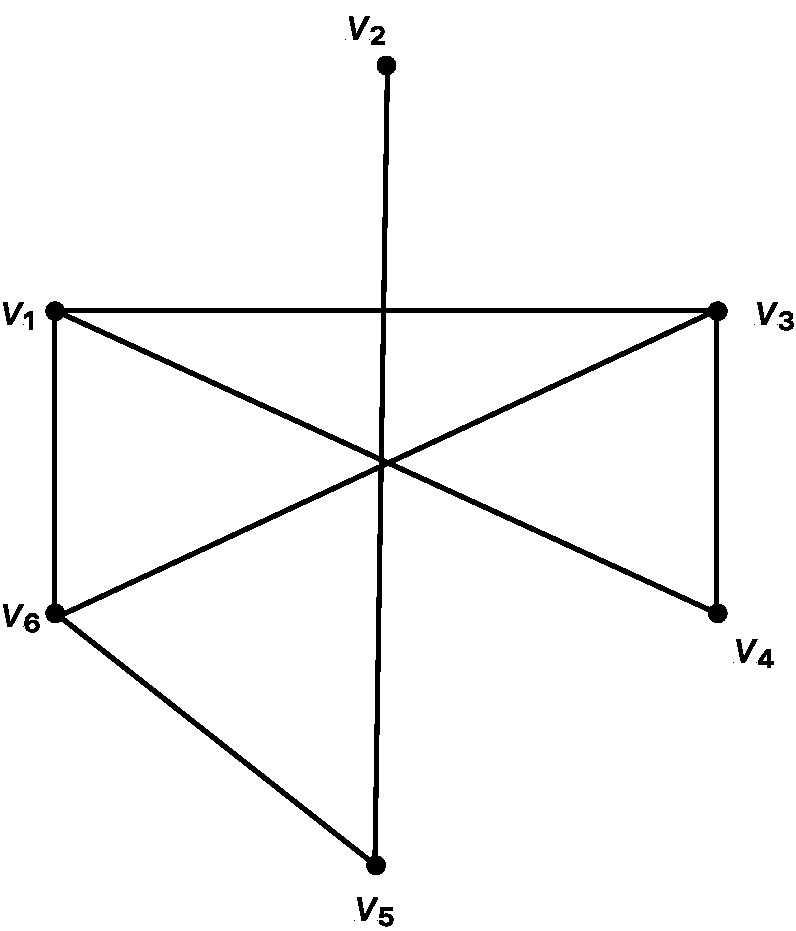
\includegraphics[scale=.8]{20_2.pdf}
\end{center}

В полученном графе степень вершины $v_1$ - три, поэтому
эйлерового цикла нет. Проверим, есть ли эйлерова цепь (может быть
максимум две вершины нечетной степени). Это условие не
выполняется, т.к. нечетные степени у вершин с номерами 1, 2, 3, 6,
следовательно и эйлеровой цепи нет.

Проведем раскраску графа.

Переупорядочим вершины в невозрастающем порядке по
локальной степени вершины. Получим:

\begin{center}
	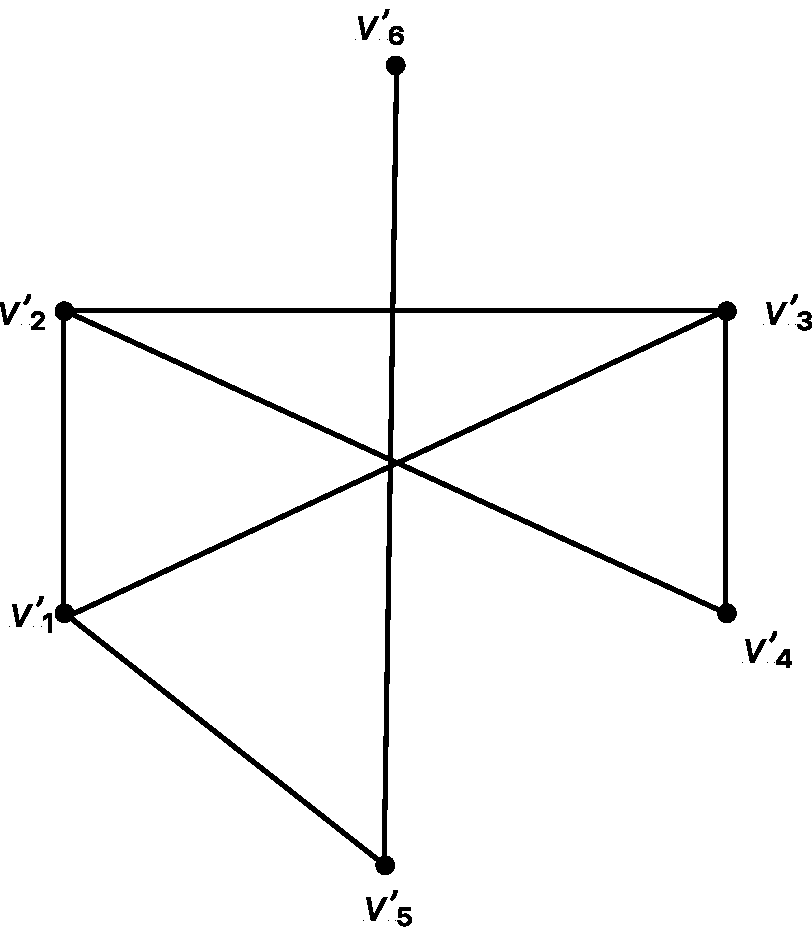
\includegraphics[scale=.8]{20_3.pdf}
\end{center}

Берем первую вершину (с самой большой локальной степенью
вершины) – это $v_1^'$. Ее покрасим в цвет 1. В этот же цвет покрасим и
все вершины, которые не являются смежными с первой вершиной, а
также между собой (это вершины $v_4^'$  и v_6^'$). Эти вершины уберем из
рассмотрения.

\begin{center}
	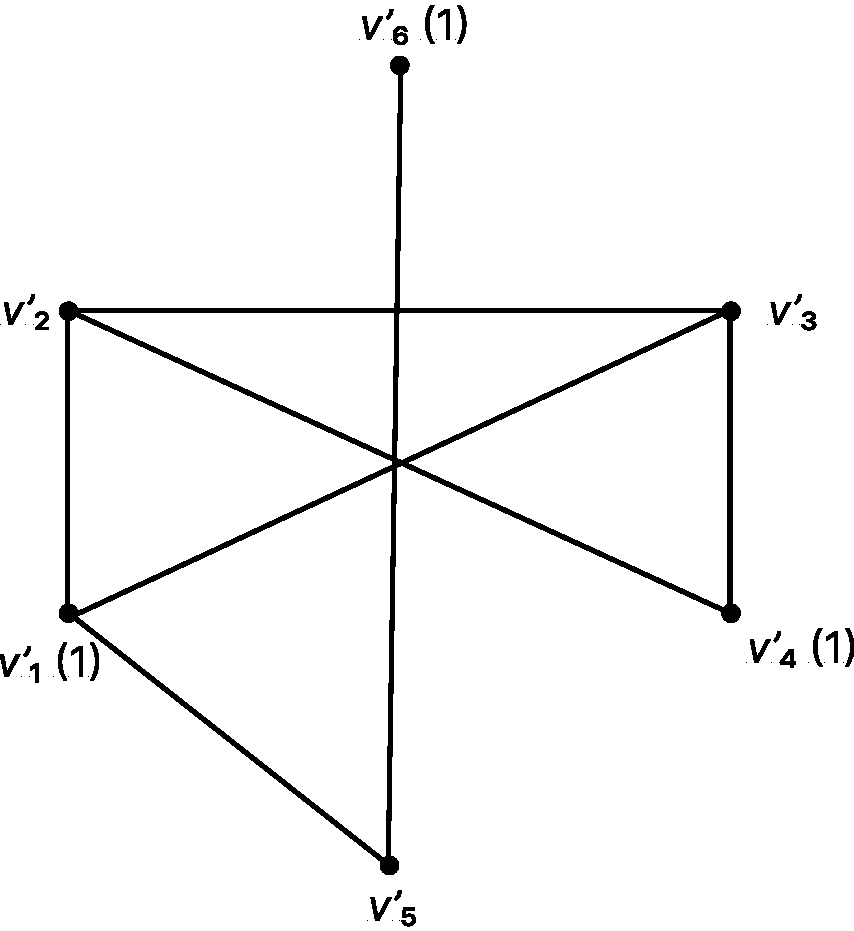
\includegraphics[scale=.8]{20_4.pdf}
\end{center}

Повторяем предыдущий шаг для нового списка вершин. Берем
первую вершину из не рассмотренных (с самой большой локальной
степенью вершины) – это $v_2^'$. Ее покрасим в цвет 2. В этот же цвет
покрасим и все вершины, которые не являются смежными с этой
вершиной, а также между собой - это только вершина $v_5^'$.
Эти вершины уберем из рассмотрения.

\begin{center}
	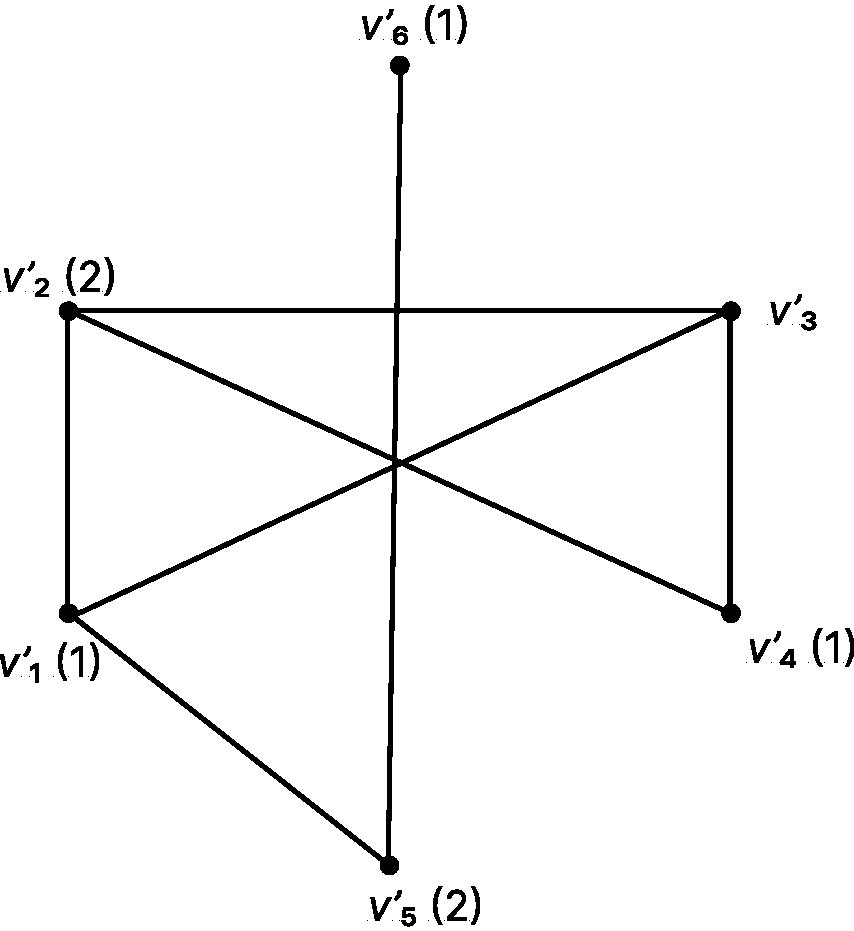
\includegraphics[scale=.8]{20_5.pdf}
\end{center}

Осталась вершина $v_3^'$. Ее покрасим в цвет 3. Раскраска завершена:

\begin{center}
	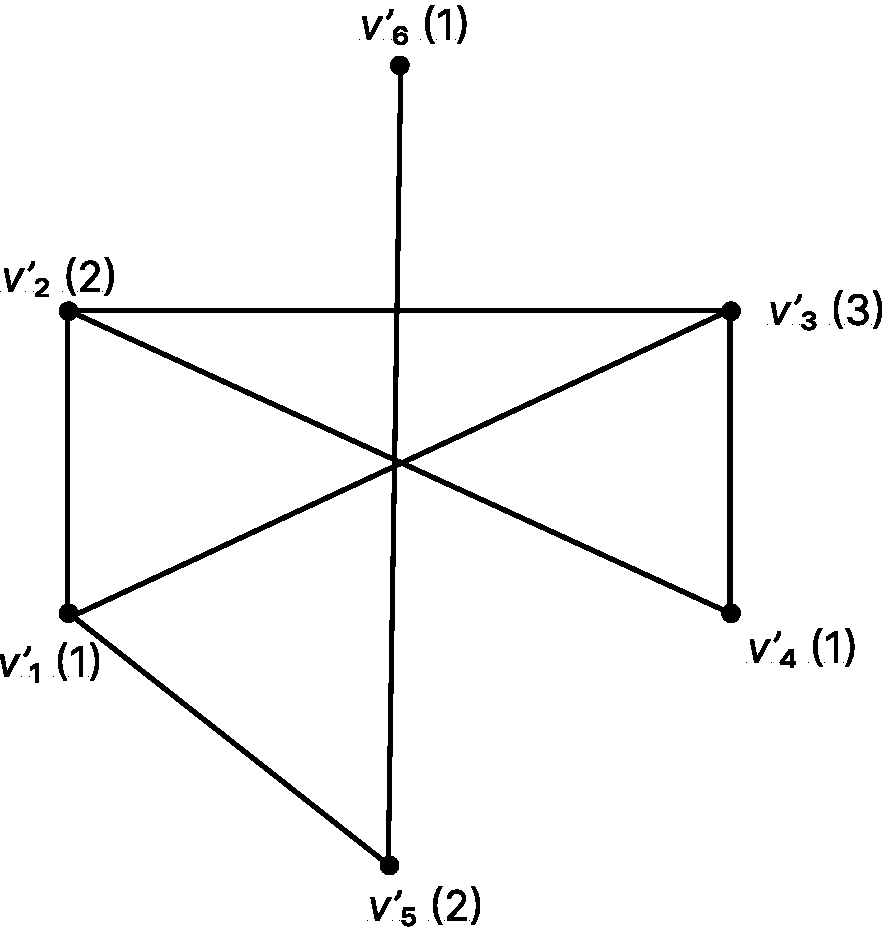
\includegraphics[scale=.8]{20_6.pdf}
\end{center}

Хроматическое число $\chi (G) = 3$, поскольку использовались только 3
цвета.

\end{document}
